% This line sets the project root file.
% !TEX root = Notes_Gauging_Defects.tex
% !TEX spellcheck = en_US

\subsection{Bimodules}

\begin{definition}
	Let $\mathcal{C}$ be a fusion category. A \textbf{left module category} over $\mathcal{C}$ is a semi-simple category $\mathcal{M}$ equipped with a left $\mathcal{C}$-\emph{action}, i.e.\ a functor $\triangleright:\mathcal{C}\times\mathcal{M}\to\mathcal{M}$ and a natural isomorphism 
		\begin{equation}
			a\triangleright(b\triangleright m)\cong(a\otimes b)\triangleright m
		\end{equation}
	which satisfies some coherence conditions that can be found in Section~7.1 of \cite{Etingof2015}. If we choose bases for all the vector spaces $\mathcal{M}(a\triangleright m,n)$, this associator can be written in terms of a tensor $L$ using string diagrams
		\begin{equation}
			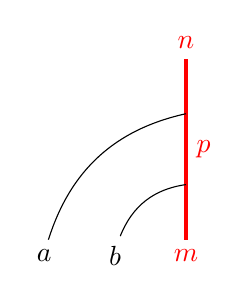
\begin{tikzpicture}[scale=0.9,baseline=(current bounding box.center)]
			\node[red](m) at (0,0) {$m$};
			\node(b) at (-1,0) {$b$};
			\node(a) at (-2,0) {$a$};
			\node[red](abm) at (0,3) {$n$};
			\draw[red,line width=0.4mm] (m) to node[right] {$p$} (abm);
			\draw (b) to [bend left] (0,1);
			\draw (a) to [bend left] (0,2);
			\end{tikzpicture}\ =\sum_q \left(L^n_{abm}\right)_{p,q}
			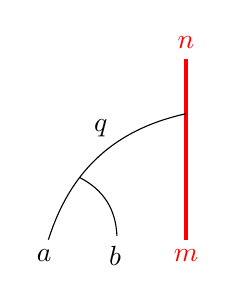
\begin{tikzpicture}[scale=0.9,baseline=(current bounding box.center)]
			\node[red](m) at (0,0) {$m$};
			\node(b) at (-1,0) {$b$};
			\node(a) at (-2,0) {$a$};
			\node[red](abm) at (0,3) {$n$};
			\node(ab) at (-1.2,1.8) {$q$};
			\draw[red,line width=0.4mm] (m) to (abm);
			\draw (b) to [bend right] (-1.5,1.1);
			\draw (a) to [bend left] (0,2);
			\end{tikzpicture},\label{eqn:L}
		\end{equation}
	where we have marked the objects of the module category in red. One can define a \textbf{right module category} over $\mathcal{C}$ in a similar way: Here, we have a semi-simple category $\mathcal{M}$ with a functor $\triangleleft:\mathcal{M}\times\mathcal{C}\to\mathcal{M}$ and a natural isomorphism
		\begin{equation}
			(m\triangleleft a)\triangleleft b\cong m\triangleleft(a\otimes b)
		\end{equation}
	(satisfying some coherence conditions), which we can represent by a tensor $R$:
		\begin{equation}
			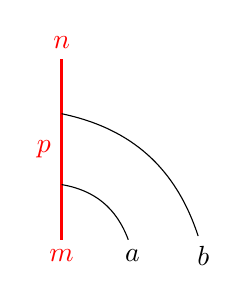
\begin{tikzpicture}[scale=0.9,baseline=(current bounding box.center)]
			\node[red](m) at (0,0) {$m$};
			\node(b) at (1,0) {$a$};
			\node(a) at (2,0) {$b$};
			\node[red](abm) at (0,3) {$n$};
			\draw[red,line width=0.4mm] (m) to node [left] {$p$} (abm);
			\draw (b) to [bend right] (0,1);
			\draw (a) to [bend right] (0,2);
			\end{tikzpicture}\ =\sum_q\left(R^n_{mab}\right)_{p,q}
			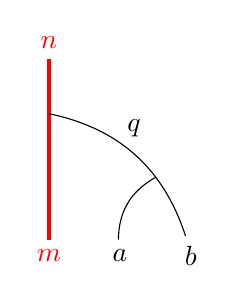
\begin{tikzpicture}[scale=0.9,baseline=(current bounding box.center)]
			\node[red](m) at (0,0) {$m$};
			\node(b) at (1,0) {$a$};
			\node(a) at (2,0) {$b$};
			\node[red](abm) at (0,3) {$n$};
			\node(ab) at (1.2,1.8) {$q$};
			\draw[red,line width=0.4mm] (m) to (abm);
			\draw (b) to [bend left] (1.5,1.1);
			\draw (a) to [bend right] (0,2);
			\end{tikzpicture}.\label{eqn:R}
		\end{equation}
	
\begin{definition}
	Let $\mathcal{C}, \mathcal{D}$ be fusion categories. A $(\mathcal{C},\mathcal{D})$-\textbf{bimodule category} (also written $\mathcal{C}\curvearrowright\mathcal{M}\curvearrowleft\mathcal{D}$) is a semi-simple category $\mathcal{M}$ that has left $\mathcal{C}$-module and right $\mathcal{D}$-module category structures, i.e.\ there are natural isomorphisms 
		\begin{align}
			a\triangleright(b\triangleright m)&\cong(a\otimes b)\triangleright m\\ 
			(m\triangleleft a)\triangleleft b&\cong m\triangleleft(a\otimes b)
		\end{align}
	that satisfy certain coherence conditions between $L$ and $R$. Additionally, there is a natural isomorphism 
		\begin{equation}
			a\triangleright(m\triangleleft b)\cong (a\triangleright m)\triangleleft b.
		\end{equation}
	As above, after choosing bases for the morphism spaces, this can be represented in terms of string diagrams with a tensor $C$:
		\begin{equation}
			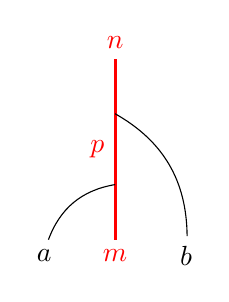
\begin{tikzpicture}[scale=0.9,baseline=(current bounding box.center)]
			\node[red](m) at (0,0) {$m$};
			\node(a) at (-1,0) {$a$};
			\node(b) at (1,0) {$b$};
			\node[red](abm) at (0,3) {$n$};
			\draw[red,line width=0.4mm] (m) to node [left] {$p$} (abm);
			\draw (a) to [bend left] (0,1);
			\draw (b) to [bend right] (0,2);
			\end{tikzpicture}\ =\sum_q\left(C^n_{amb}\right)_{pq}
			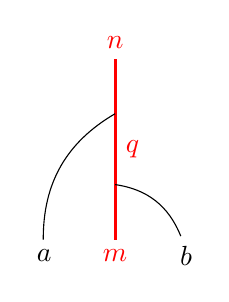
\begin{tikzpicture}[scale=0.9,baseline=(current bounding box.center)]
			\node[red](m) at (0,0) {$m$};
			\node(a) at (-1,0) {$a$};
			\node(b) at (1,0) {$b$};
			\node[red](abm) at (0,3) {$n$};
			\draw[red,line width=0.4mm] (m) to node [right] {$q$} (abm);
			\draw (b) to [bend right] (0,1);
			\draw (a) to [bend left] (0,2);
			\end{tikzpicture}.
		\end{equation}
\end{definition}

\end{definition}